Figure~\ref{fig:workflow} summarizes the system configuration and data flow, Table~\ref{tab:design} summarizes the benchmark design, Figure~\ref{fig:ja-ranking} shows the Japanese human-alignment ranking, Figure~\ref{fig:drift} shows cross-language drift relative to Japanese, Table~\ref{tab:primary} reports the core summary statistics, and Figure~\ref{fig:tradeoff} visualizes the two-axis screening view.

\textbf{Japanese human alignment.} In the primary Japanese condition, Claude Sonnet 4.5 achieved the lowest mean absolute error (MAE) to the human reference (20.026), followed by DeepSeek V3.2 (20.100), Qwen3.6 Plus (20.744), GPT-5.4 (21.113), and Grok 4.20 (21.410), whereas Gemini 2.5 Pro showed the largest error (28.952). The spread between the best and worst models was therefore 8.926 points. At the same time, the top four models were tightly clustered within only 1.087 MAE points, indicating that model screening would be sensitive to relatively small calibration differences within the stronger half of the panel.

\begin{figure*}[t]
\centering
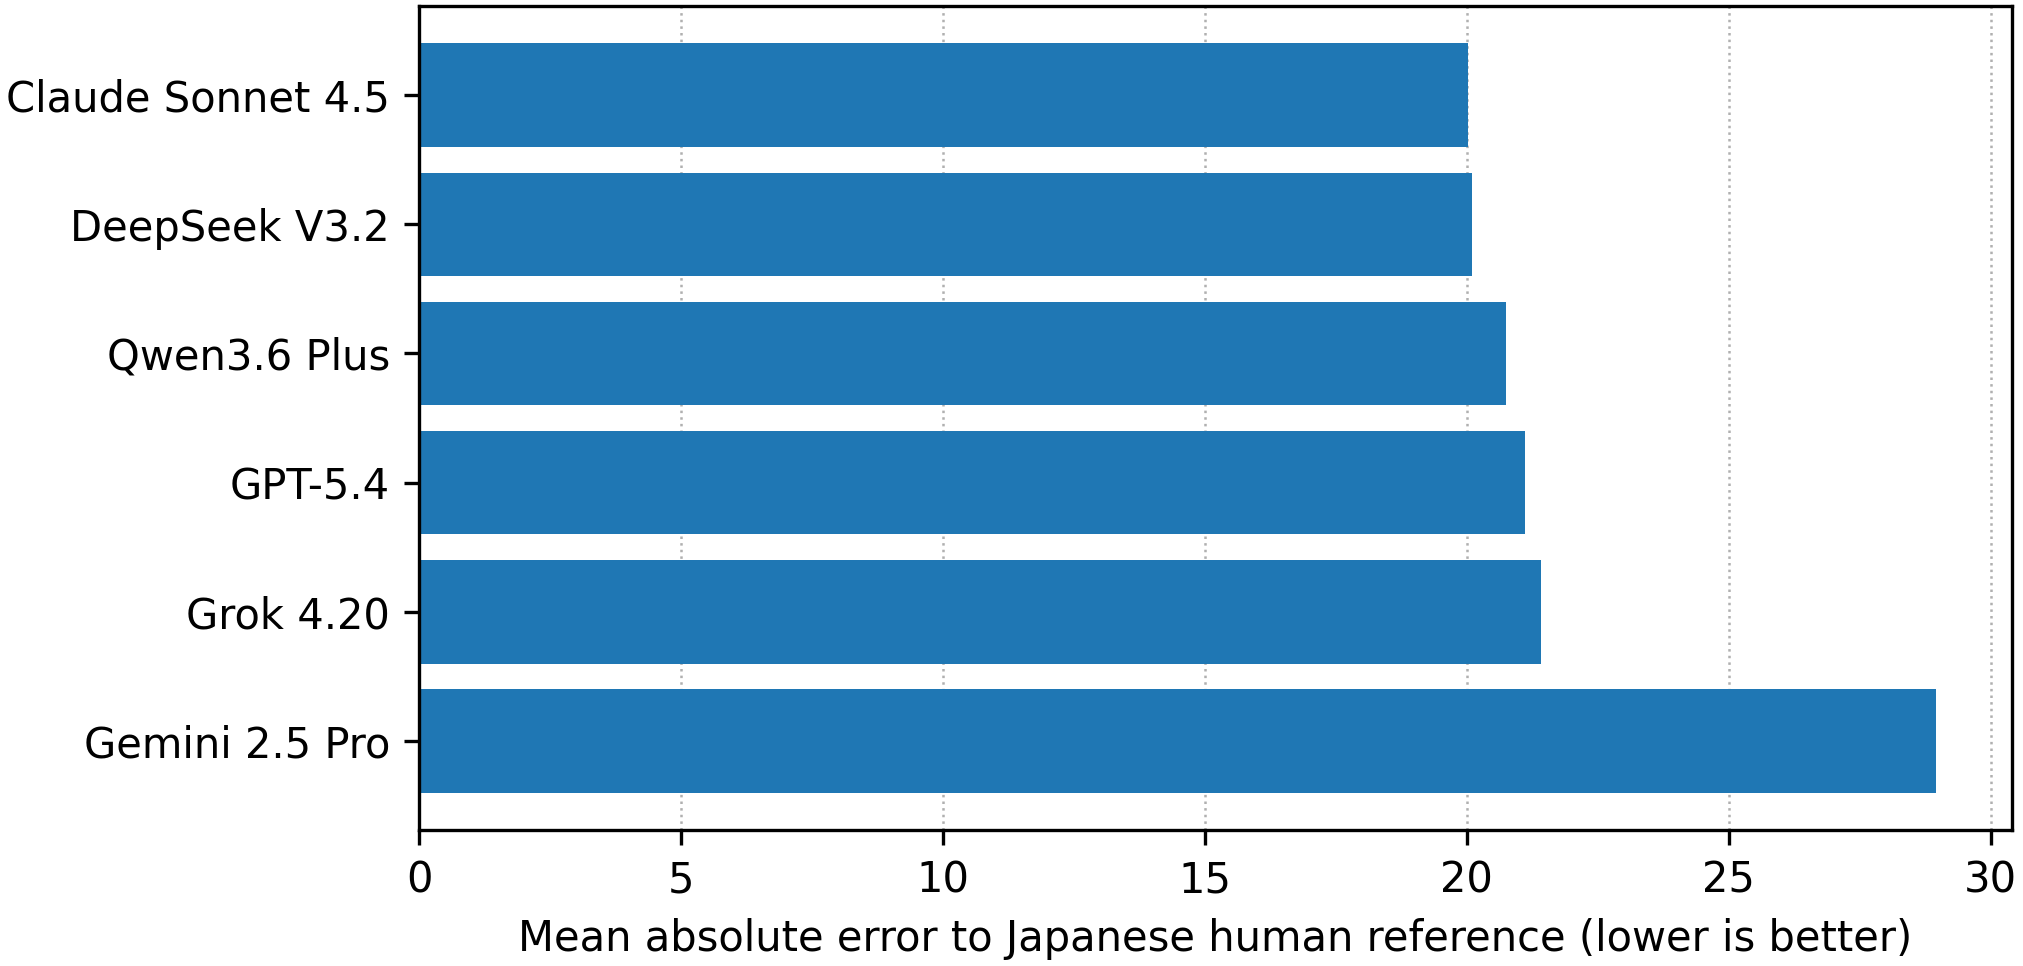
\includegraphics[width=0.94\textwidth]{fig/figure2_ja_ranking.pdf}
\caption{Japanese human-alignment ranking of the six selected models under the neutral-reader condition. Models are ordered by mean absolute error (MAE) to the Japanese human reference; lower values indicate closer agreement with human VAS judgments. Correlation coefficients are reported separately in Table~\ref{tab:primary}.}
\label{fig:ja-ranking}
\end{figure*}

GPT-5.4 yielded both the highest Pearson correlation with the Japanese human profile ($r = 0.475$) and the highest Spearman rank correlation ($\rho = 0.441$). This split is important because absolute calibration and rank-order agreement should be distinguished rather than collapsed into a single score. Claude Sonnet 4.5 was the closest in absolute intensity level, whereas GPT-5.4 best preserved relative ordering across the 12 human-reference cells.

\textbf{Cross-language robustness.} For cross-language robustness, Qwen3.6 Plus exhibited the smallest average drift relative to Japanese ($\bar{D}=3.346$), followed closely by GPT-5.4 ($\bar{D}=3.354$) and Gemini 2.5 Pro ($\bar{D}=4.729$). By contrast, DeepSeek V3.2 showed the largest average drift ($\bar{D}=6.396$), with the largest single-language drift observed in its English condition (7.875). Across all models and secondary languages, drift ranged from 2.983 to 7.875 points.

\begin{figure*}[t]
\centering
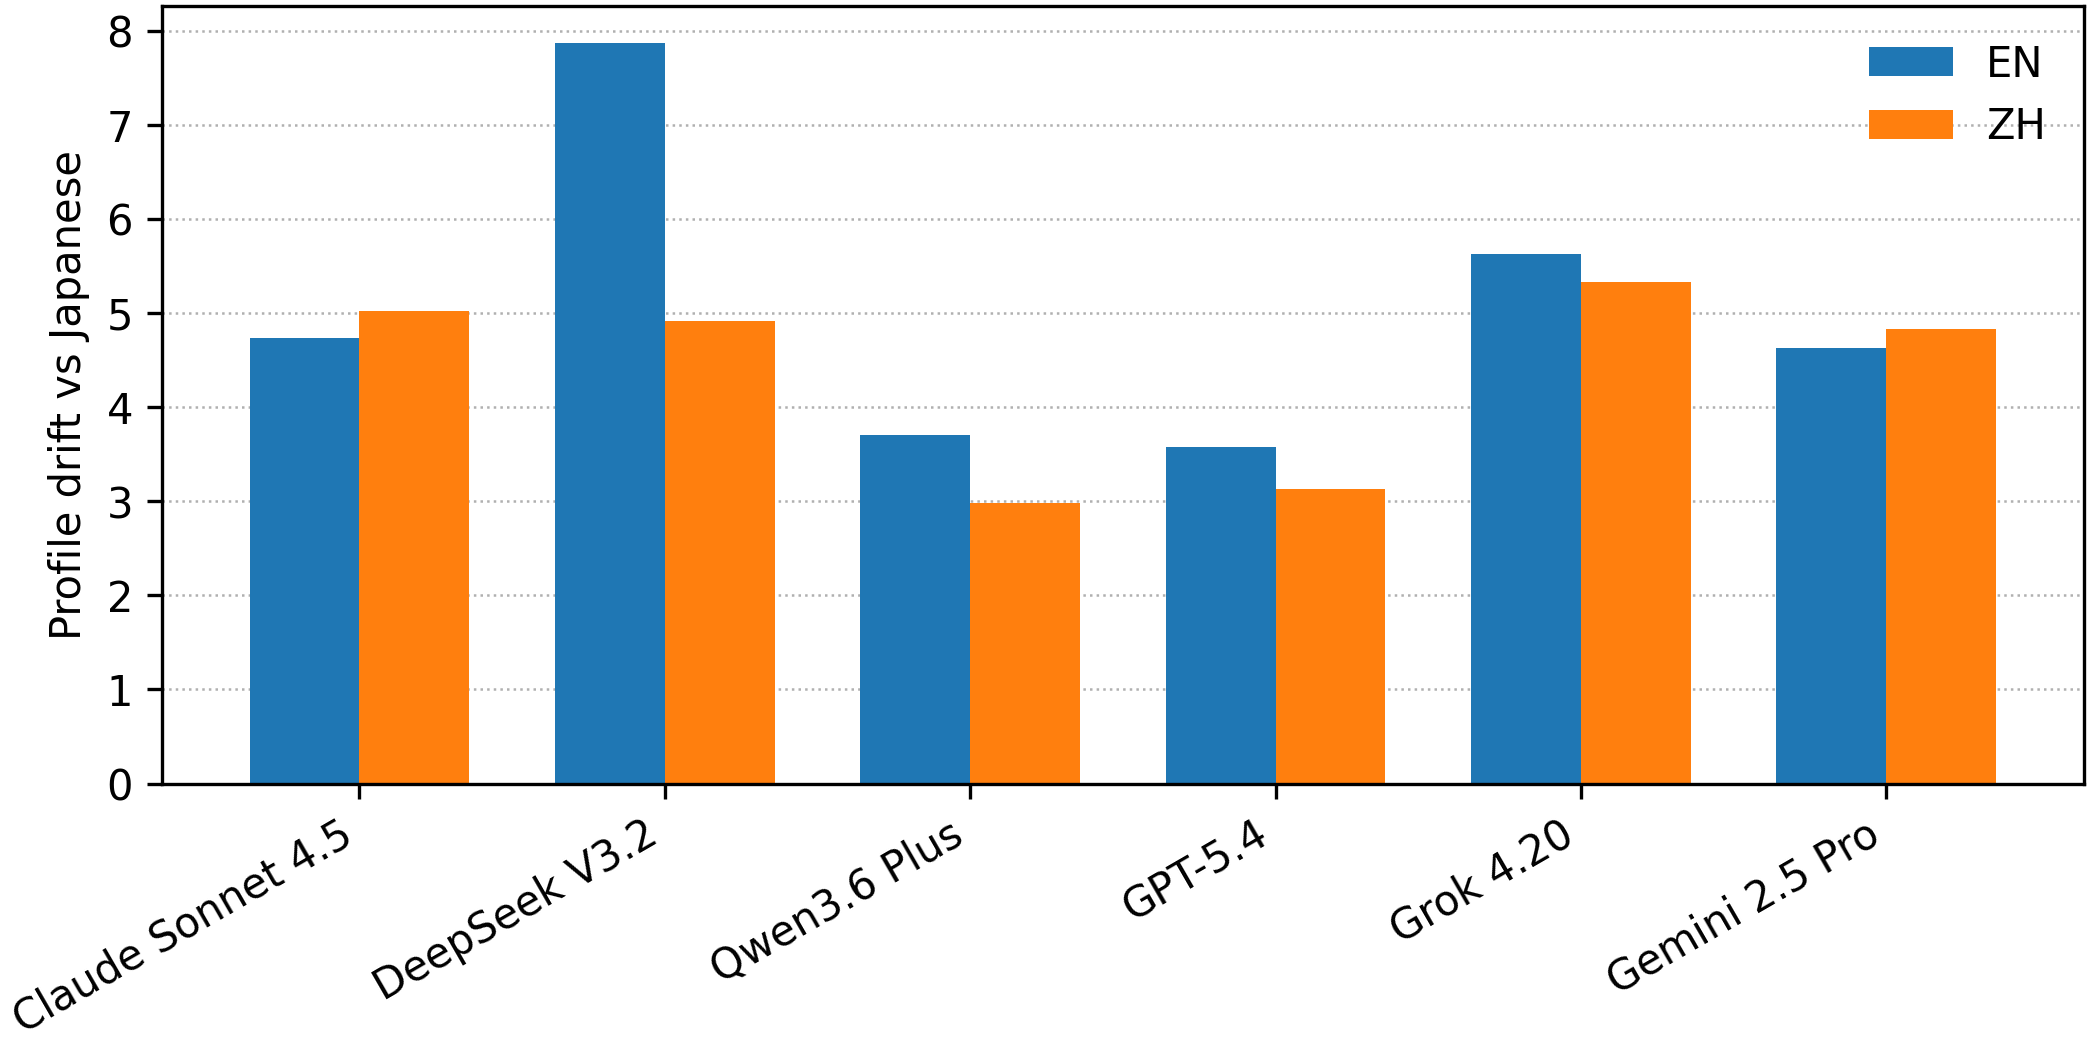
\includegraphics[width=0.94\textwidth]{fig/figure3_cross_language_drift.pdf}
\caption{Cross-language drift relative to Japanese for the six selected models under the neutral-reader condition. Drift is defined as the mean absolute difference between a model's English or Chinese story-by-emotion score profile and the same model's Japanese profile. Smaller values indicate greater cross-language robustness.}
\label{fig:drift}
\end{figure*}

The English condition was slightly less stable on average than the Chinese condition in this six-model panel: mean English drift was 5.024, whereas mean Chinese drift was 4.371. That difference is descriptive rather than inferential, but it still shows why robustness should not be assumed to be symmetric across translated conditions.

\begin{table*}[t]
\caption{Primary quantitative summary of Japanese human alignment and cross-language drift for the six selected models.}
\label{tab:primary}
\centering
\small
\begin{tabular}{lrrrrrr}
\toprule
Model & JA MAE & JA Pearson $r$ & JA Spearman $\rho$ & EN drift & ZH drift & Avg drift \\
\midrule
Claude Sonnet 4.5 & 20.026 & 0.442 & 0.252 & 4.733 & 5.025 & 4.879 \\
DeepSeek V3.2 & 20.100 & 0.459 & 0.301 & 7.875 & 4.917 & 6.396 \\
Qwen3.6 Plus & 20.744 & 0.374 & 0.214 & 3.708 & 2.983 & 3.346 \\
GPT-5.4 & 21.113 & 0.475 & 0.441 & 3.575 & 3.133 & 3.354 \\
Grok 4.20 & 21.410 & 0.305 & 0.112 & 5.625 & 5.333 & 5.479 \\
Gemini 2.5 Pro & 28.952 & 0.261 & 0.112 & 4.625 & 4.833 & 4.729 \\
\bottomrule
\end{tabular}
\end{table*}

\textbf{Two-axis screening view.} The Japanese ranking and the drift ranking are related but not identical. Claude Sonnet 4.5 is the best-calibrated model in Japanese, whereas Qwen3.6 Plus shows the smallest average cross-language drift. Gemini 2.5 Pro has the largest Japanese MAE, while DeepSeek V3.2 has the largest average drift. Figure~\ref{fig:tradeoff} makes this separation explicit by plotting Japanese human-alignment MAE against average EN/ZH drift.

\begin{figure}[t]
\centering
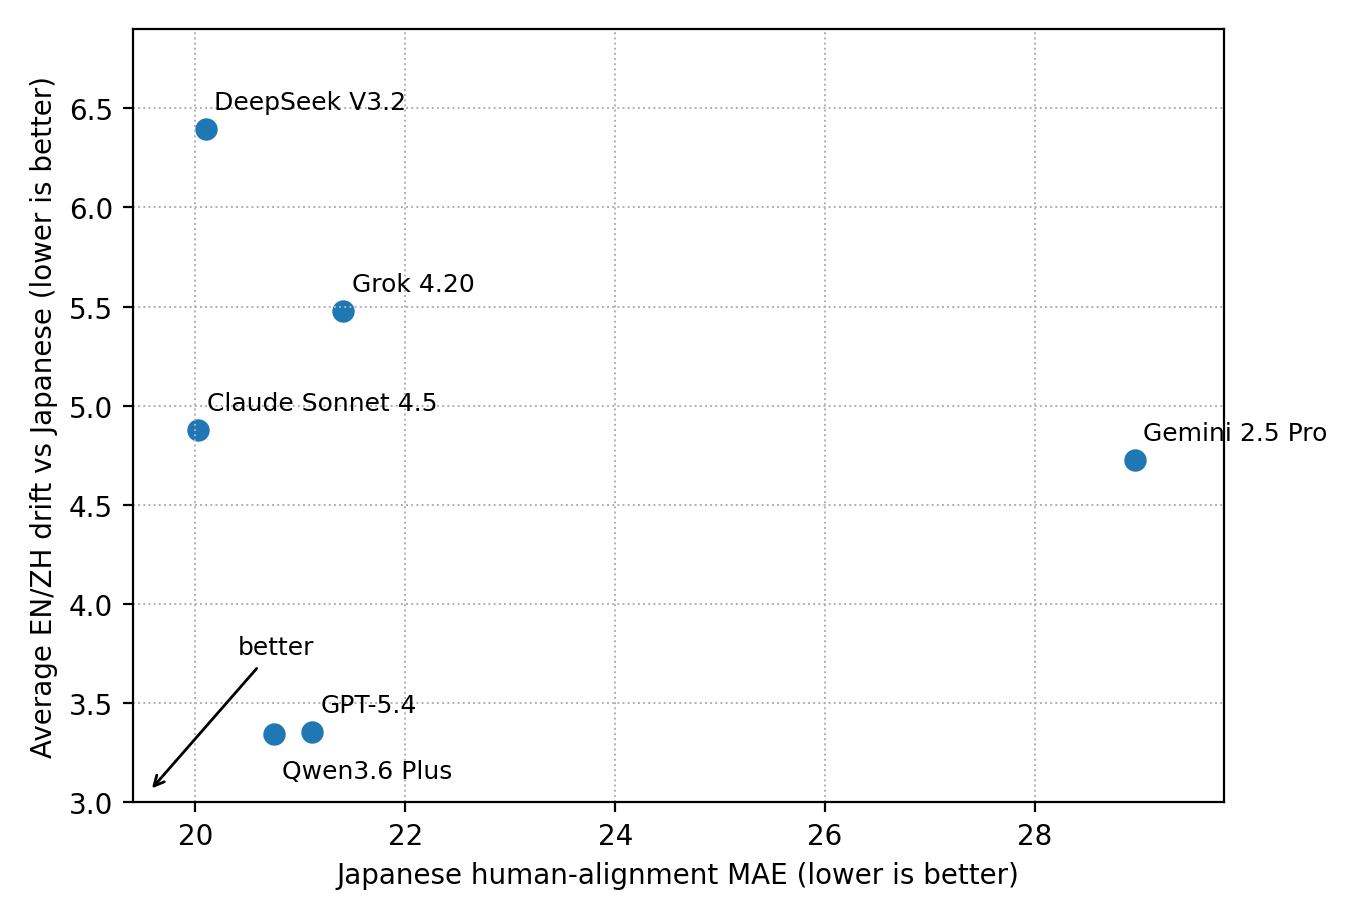
\includegraphics[width=0.98\columnwidth]{fig/figure4_alignment_vs_avg_drift.pdf}
\caption{Two-axis screening view of the benchmark. The horizontal axis shows Japanese human-alignment MAE and the vertical axis shows average EN/ZH drift relative to Japanese. The lower-left region is preferable when both primary-language calibration and multilingual robustness matter.}
\label{fig:tradeoff}
\end{figure}

No single model dominates both axes. Claude Sonnet 4.5 is strongest on the primary human-grounded endpoint, Qwen3.6 Plus and GPT-5.4 are strongest on multilingual stability, and Gemini 2.5 Pro shows that moderate robustness does not compensate for weak primary-language alignment. This separation is important for deployment-oriented evaluation: a model may align relatively well with human intensity levels in the primary language while showing different stability under translation, or vice versa.
